\section{Comparison and Discussion}
\label{sec:comparison}
\emph{In short: the frequentist and Bayesian analyses give the same value, uncertainty and coverage for $\Araw$ because they use the same likelihood and the data constrain it well; they differ in what the numbers mean and in the hypothesis tests, and the machine-learning selection confirms the result without improving it.}

\subsection{Summary of the Three Approaches}
\label{sec:comparison_summary}
\begin{table*}[t]
\centering
\small
\begin{tabular}{p{2.6cm}p{4.9cm}p{4.9cm}p{4.2cm}}
\toprule
 & Frequentist (Sec.~\ref{sec:frequentist}) & Bayesian (Sec.~\ref{sec:bayesian}) & ML-assisted (Sec.~\ref{sec:ml}) \\
\midrule
Question & Which value of $A$ makes the data most probable, and which values are not rejected? & What is the distribution of $A$ given the data and the prior? & Does a data-driven selection change $\Araw$ or the mass spectrum? \\
Estimate & Maximum likelihood, $-0.0441$ & Posterior median, $-0.0443$ (mode $-0.0441$) & Same fits after a score cut: $-0.0447$ (freq.), $-0.0451$ (Bayes) \\
Interval (68\%) & $[-0.0526,-0.0356]$ (profile likelihood, Minos) & $[-0.0528,-0.0358]$ (credible, equal-tailed) & Statistical spread of a nested sample \\
Test of $A=0$ & $q(0)\simeq27$, $p=2.05\times10^{-7}$, $5.2\sigma$ & $BF_{01}\approx1.1\times10^{-4}$ (Savage-Dickey) & $5.2\sigma$ in both samples \\
Validation of the interval & $1000$ bootstrap replicas: $68.4\pm1.5\%$; $985$ toys: $70\pm1\%$ ($68\%$), $95\pm1\%$ ($95\%$) & $200$ toys: $0.65\pm0.03$ ($68\%$), $0.93\pm0.02$ ($95\%$) & -- \\
Goodness of fit & $\chi^2/\mathrm{ndof}\approx160/88$ ($10\,\MeV$ bins); $441.7/388$, $p=0.031$ ($2.5\,\MeV$ bins) & $164.1/88$ ($p=1.6\times10^{-6}$); posterior predictive check & AUC of the classifiers, calibration \\
Computing time & one joint fit with Minos $\simeq19\,$s; $1000$ bootstrap fits $\simeq49\,$min & one chain ($25{,}000$ steps, 32 walkers) $\simeq8\,$min; $200$ toys of $12{,}000$ steps & training of six classifiers, hyperparameter search \\
\bottomrule
\end{tabular}
\caption{Frequentist, Bayesian and machine-learning-assisted analyses compared on the same candidates ($\Araw$, statistical uncertainties only). Computing times are indicative, on one laptop.}
\label{tab:comparison}
\end{table*}

Table~\ref{tab:comparison} puts side by side what each approach was used for, what it gave and how it was validated.



\subsection{Numerical Agreement}
\label{sec:comparison_numbers}
The two fits of the same model agree to the precision of the quoted digits: the estimates differ by $0.0002$ ($0.02$ standard deviations), the uncertainties are both $0.0085$, the $68\%$ and $95\%$ intervals differ by at most $0.0002$, and the shifts of the thirteen systematic variants agree within $0.0005$, with the same group uncertainties for the window ($0.0014$) and the preselection ($0.0058$) and slightly different ones for the background ($0.0037$ against $0.0040$) and the signal model ($0.0002$ against $0.0006$), so that the total systematic uncertainties are $0.0070$ and $0.0072$ (Sec.~\ref{sec:syst}). A third estimate, by sideband subtraction (counting in the signal region after removing the background expected from the sideband fit), gives $-0.0503\pm0.0083$, which differs from the nominal value by $0.006$, less than one standard deviation, on the same candidates. This is expected, and it is not by itself a validation of the model. With $\sim2\times10^4$ candidates and flat priors the posterior is proportional to the likelihood, the likelihood is close to a Gaussian in $A$, and the posterior mode coincides with the maximum-likelihood estimate; the posterior median, the posterior mean and the mode differ by less than $2\times10^{-4}$. What the agreement does show is that neither the sampling (MCMC) nor the asymptotic approximations (Hesse, Wilks) introduce a bias: the Bayesian intervals have the coverage of the frequentist ones (Sec.~\ref{sec:bayes_toymc}) and the profile-likelihood interval has the coverage assumed by Wilks' theorem (Sec.~\ref{sec:freq_coverage}).

The agreement does not extend to the validity of the model itself. Both methods describe the same spectrum with the same Gaussian signal and double-exponential background, and neither reaches $\chi^2/\mathrm{ndof}\approx1$ (Sec.~\ref{sec:bayes_gof}); what protects $\Araw$ is that its value does not depend on the signal shape (shift $-0.0002$ with a Crystal Ball) and that the background treatment, the largest model dependence, is included in the systematic uncertainty.

\subsection{Where the Approaches Differ}
\label{sec:comparison_differ}
\emph{Meaning of the interval.} The credible interval $[-0.0528,-0.0358]$ states that, given the data and the prior, $A$ lies in it with $68\%$ probability; the confidence interval $[-0.0526,-0.0356]$ is the set of values that the data do not reject at the $32\%$ level, and the $68\%$ is the fraction of repeated experiments in which such an interval contains the true value. The numbers are the same here; the statements are not, and only the second is a property of the procedure that can be checked by repeating the experiment, which is what the bootstrap and toy checks did.

\emph{Hypothesis test.} The simplest test, the exact binomial test of $N^-=N^+$ on all candidates of the window, gives $6.1\sigma$ ($p=1.3\times10^{-9}$, $A_{\mathrm{count}}=-0.0432\pm0.0071$); it sees the asymmetry of signal and background together and does not use the mass. The frequentist test of the fit gives a $p$-value, $2\times10^{-7}$ ($Z=\sqrt{q(0)}=5.2\sigma$ in the two-sided convention; the one-sided $Z=\Phi^{-1}(1-p)$ would give $5.06\sigma$, Appendix~\ref{sec:appendix_freq}), which does not depend on the prior and is not the probability of $A=0$; its size and power were verified with pseudo-experiments (Sec.~\ref{sec:validation_power}). In particle physics a significance of $5\sigma$ is the conventional threshold for a discovery claim, chosen to limit the effect of multiple testing and of unforeseen systematic effects; the $5.2\sigma$ found here crosses it, but it refers to a raw asymmetry that includes production and detection effects (Sec.~\ref{sec:comparison_published}), and is not a discovery of CP violation. The Bayes factor, $BF_{10}\approx9\times10^3$, compares the evidence of $A$ free and $A=0$ and depends on the prior width: with $A\in(-0.3,0.3)$ instead of $(-1,1)$ it decreases by a factor $3.3$. For $A$ the two give the same conclusion. For the background asymmetry, $A_b=-0.040\pm0.018$, they would lead to different statements: a $2.3\sigma$ deviation from zero, which a frequentist test would call a hint, and $BF_{01}\approx3.5$, a mild preference for $A_b=0$ because a free parameter with a prior of width two is penalized (Sec.~\ref{sec:bayes_factor}). Neither is wrong; they answer different questions.

\emph{Goodness of fit.} The same fit of the same data gives $\chi^2/\mathrm{ndof}=441.7/388$ ($p=0.031$) in $2\times200$ bins of $2.5\,\MeV$ and $\approx160/88$ ($p\approx5\times10^{-6}$) in $2\times50$ bins of $10\,\MeV$ (the Bayesian fit, $164.1/88$, $p=1.6\times10^{-6}$, uses the second binning). The misfit is at the scale of $\sim10\,\MeV$, the flanks of the peak, and is diluted in narrow bins where Poisson fluctuations dominate; the $p$-value of a binned $\chi^2$ is a property of the binning as much as of the model. The Bayesian analysis adds the posterior predictive check, which accounts for the posterior uncertainty of the parameters and shows that the misfit is concentrated in the $B^+$ sample (Sec.~\ref{sec:bayes_gof}).

\emph{Nuisance parameters.} The frequentist analysis profiles the eleven nuisance parameters, the Bayesian one marginalizes them. The two differ when the likelihood is far from Gaussian or the prior is informative; here $A$ is almost uncorrelated with the others (largest correlation $-0.17$, with $A_b$), and the results coincide.

\emph{Validation.} The Bayesian toys are generated from the fitted model, which makes them a closure test; the bootstrap replicas of the frequentist check are resampled from the data and carry the features that the model does not describe. That both give the nominal coverage supports the interval, but they test different things (Sec.~\ref{sec:freq_coverage}).

\subsection{Machine Learning and the Fits}
\label{sec:comparison_ml}
The machine-learning selection was used as a cross-check of the fits, not as a replacement. A cut on the gradient-boosting score at $0.5$ keeps $92\%$ of the fitted signal and $36\%$ of the background and does not change $\Araw$ beyond its expected statistical spread, with both inference methods ($-0.0451\pm0.0087$ Bayesian, $-0.0447\pm0.0086$ frequentist, against $-0.0443$ and $-0.0441$ for the full window). It does not improve the precision, $0.0087$ against $0.0085$, because the nominal sample contains little background. In a sample with a looser kaon identification ($33{,}328$ candidates) the classifier raises the purity from $94\%$ to $99\%$ and reduces $\sigma(\Araw)$ from $0.0072$ to $0.0070$ at best, and it cannot remove the misidentified decays that move $\Araw$ to $-0.055$: they peak under the signal, and weak labels derived from the mass spectrum mark them as signal-like (Sec.~\ref{sec:ml_stability}). The useful role of the machine-learning module is therefore that of a consistency test of the asymmetry under a different event selection, and the partition of the Dalitz plane that it provides (below). Gaining precision or controlling the peaking background would require labels that carry information beyond the mass, such as simulation.

\subsection{Local Asymmetries: Fixed Binning and $K$-Means}
\label{sec:comparison_local}
Two partitions of the Dalitz plane were used, a fixed $8\times8$ grid (Sec.~\ref{sec:dalitz}) and an adaptive $K$-means partition with $K=8$ (Sec.~\ref{sec:ml_kmeans}). Both find that the asymmetry is not uniform: $\chi^2=80.8$ for $31$ degrees of freedom for the grid and $46.4$ for $7$ for $K$-means ($p=3\times10^{-6}$ and $7\times10^{-8}$). Both place the negative local asymmetry at low $m^2_{\mathrm{lo}}$ and intermediate $m^2_{\mathrm{hi}}$ ($A=-0.128\pm0.018$ in the region of the two significant bins, $-0.127\pm0.017$ in the most significant cluster) and positive deviations at high $m^2_{\mathrm{hi}}$. The two partitions have different bins, so the numbers are not independent, and the $K$-means $p$-value benefits from the larger bins; the agreement is in the pattern. In the region defined by the published analysis, fixed before looking at the data, both fits give a compatible value ($-0.234\pm0.025$ Bayesian, $-0.237\pm0.025$ frequentist, $9.4\sigma$ from zero) with $-0.239\pm0.020$. All local numbers are counting asymmetries or fits of the integrated mass spectrum in a region, with no background subtraction by event weights and no correction for detection asymmetries (Sec.~\ref{sec:limitations}).

\subsection{Comparison with the Published Analysis}
\label{sec:comparison_published}
The published analysis of the same data~\cite{lhcb_cpv_2013} finds $\Araw=-0.060\pm0.007$ with $22{,}119\pm164$ signal candidates, against $-0.0441\pm0.0085$ and $15{,}328\pm133$ here. The two differ in the sample (the Open Data record is a preselected subset, reduced to $23{,}895$ candidates by the identification requirement alone) and in the model, which includes a Cruijff signal, partially reconstructed four-body decays and a misidentified peaking background from simulation. With the same $D^0$ veto as the published selection the Bayesian fit gives $-0.0496\pm0.0088$, within one standard deviation of the quadrature sum of the two uncertainties ($0.93\sigma$), although the samples overlap and the selections differ.

The raw asymmetry is not the CP asymmetry. The two are related by $\ACP\approx\Araw-A_P-A_D$ (Eq.~\eqref{eq:acp}) and, in the published analysis, the correction obtained from $B^\pm\to J/\psi K^\pm$ decays and from the acceptance moves the result from $-0.060$ to $-0.043\pm0.009\pm0.003\pm0.007$ ($3.7\sigma$)~\cite{lhcb_cpv_2013}, i.e.\ by $+0.017$, of the order of two statistical uncertainties of this work. A correction of that size cannot be assumed for a different selection, and the $5.2\sigma$ of this work is the significance of a nonzero raw asymmetry, which includes the production asymmetry of $B^\pm$ mesons and the different interaction of $K^+$ and $K^-$ with the detector, not a significance of CP violation. A later measurement on a larger data set gives $\ACP=-0.037\pm0.002\pm0.002\pm0.003$ ($8.5\sigma$)~\cite{lhcb_cpv_prd2023,lhcb_cpv_paper}. Our result is consistent in sign and size with these values, which is what can be said without the control channel, absent from this record.

\subsection{Bayesian and Frequentist Intervals at Low Statistics}
\label{sec:bayes_lowstat}
\emph{In short: credible and confidence intervals coincide for $\sim2\times10^4$ candidates with flat priors, and stay equal, in value and coverage, down to $50$ candidates.}
With $\sim$$2\times10^4$ candidates the posterior is Gaussian and, with flat priors, the Bayesian and frequentist results coincide by construction (Sec.~\ref{sec:bayes_posterior}). To find where they could differ, the same likelihood was analysed with both methods on pseudo-datasets of $N=50$, $150$, $500$ and $2000$ candidates, $300$ for each size. The model is the six-parameter one of Sec.~\ref{sec:bayes_minimal} (Gaussian signal, one exponential background shared by the charges), which stays identifiable down to a few tens of events; the parameters are those of its fit to the data, with the yields rescaled. Each replica is analysed with the MCMC (median and equal-tailed credible intervals) and by maximum likelihood with \texttt{iminuit} (Hesse intervals, and Minos intervals from the profile likelihood and Wilks' theorem).

\begin{figure*}[t]
\centering
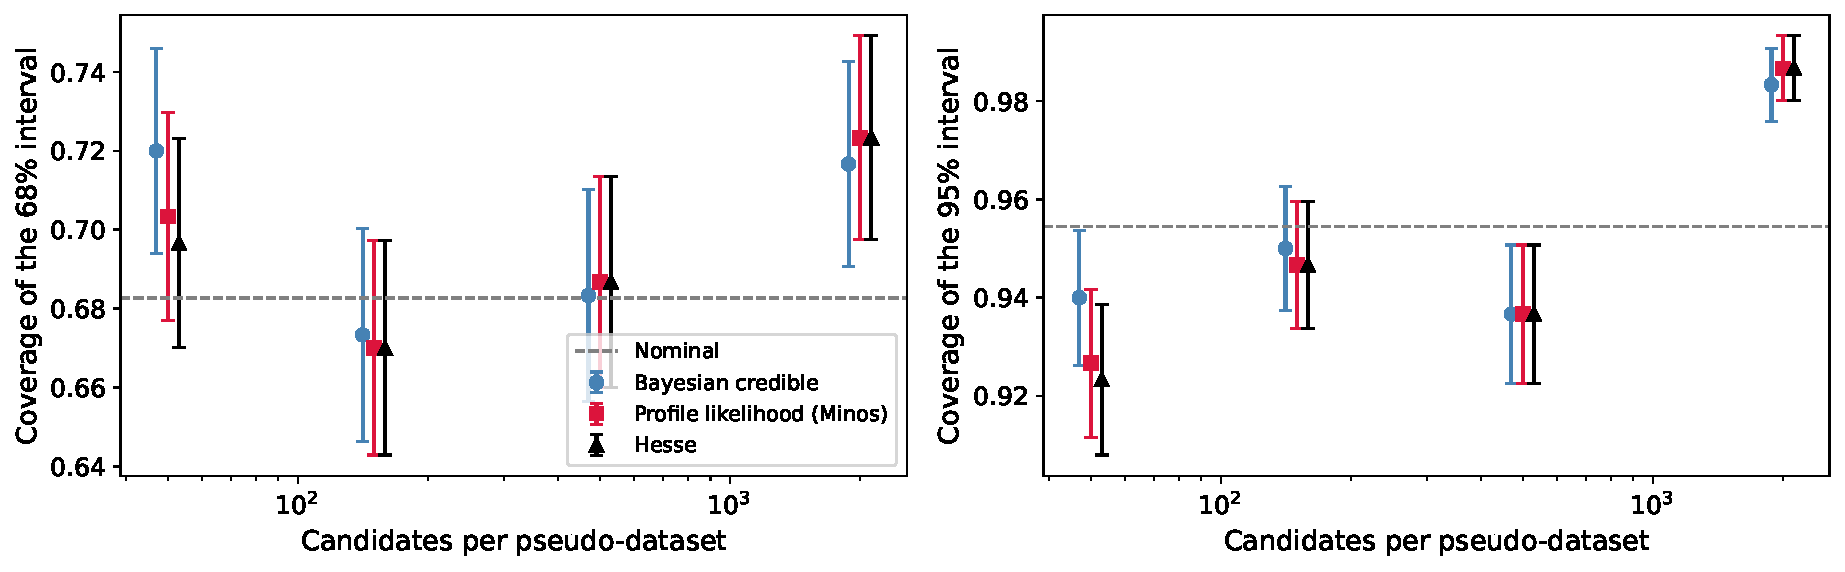
\includegraphics[width=0.95\textwidth]{figures/bayes_nominal_lowstat.pdf}
\caption{Coverage of the (a) 68\% and (b) 95\% intervals on $A$ vs the number of candidates, for the Bayesian credible interval, the profile-likelihood (Minos) interval and the Hesse interval of the same likelihood; 300 pseudo-datasets per point, binomial uncertainties. The dashed lines mark the nominal coverage ($1\sigma$, $2\sigma$; the Bayesian 95\% interval is the 2.5--97.5\% one).}
\label{fig:bayes_lowstat}
\end{figure*}

The two methods agree at every size (Fig.~\ref{fig:bayes_lowstat}). The coverages of the three intervals are compatible with nominal and with each other, the posterior median and the maximum-likelihood estimate differ on average by $5\%$ of the statistical uncertainty at $N=50$ and by less above, and the credible intervals stay symmetric (at $N=50$ the shortest chain is only $\approx10$ autocorrelation times long, so the Monte Carlo error on the interval endpoints is larger there). The asymmetry is a ratio of Poisson yields, whose likelihood is close to Gaussian already with a few tens of signal events: in this problem flat-prior credible intervals and profile-likelihood confidence intervals give the same answer, and Wilks' theorem holds, down to $N=50$. The two approaches differ in what the interval means and in hypothesis testing (Sec.~\ref{sec:bayes_factor}), not in the numbers. At $N=2000$ all three intervals over-cover slightly ($0.98$--$0.99$ for the 95\% interval); since the effect is the same for the three methods, it is a feature of this set of replicas rather than of either inference.


